\documentclass{article}[12pt]

\usepackage{amsmath}
\usepackage{graphicx}
\usepackage{float}
\usepackage{xcolor}
\usepackage{listings}
\usepackage{url}
\usepackage{amsmath}
\usepackage{geometry}
\usepackage{tcolorbox}
\usepackage{amssymb}
\usepackage{url}
 \geometry{
 a4paper,
 total={170mm,257mm},
 left=20mm,
 top=20mm,
 }
 
 \setlength\parindent{0pt}
 
 \definecolor{mGreen}{rgb}{0,0.6,0}
\definecolor{mGray}{rgb}{0.5,0.5,0.5}
\definecolor{mPurple}{rgb}{0.58,0,0.82}
\definecolor{backgroundColour}{rgb}{0.95,0.95,0.92}

\lstdefinestyle{CStyle}{
    backgroundcolor=\color{backgroundColour},   
    commentstyle=\color{mGreen},
    keywordstyle=\color{magenta},
    numberstyle=\tiny\color{mGray},
    stringstyle=\color{mPurple},
    basicstyle=\footnotesize,
    breakatwhitespace=false,         
    breaklines=true,                 
    captionpos=b,                    
    keepspaces=true,                 
    numbers=left,                    
    numbersep=5pt,                  
    showspaces=false,                
    showstringspaces=false,
    showtabs=false,                  
    tabsize=2,
    language=C
}

\begin{document}

\begin{center}
\huge{\textbf{CTmeasure - ATMega328p}}
\end{center}

\begin{center}
\textbf{Author: nmt@nt-com.org}
\end{center}

\abstract{This document describes the CTmeasure project ported to the 8-bit ATMega328p microcontroller. With the proof of concept working on the STM32 platform, the next step is porting the project to a smaller controller. As I only have a ATMega328p at my disposal, I chose this microcontroller for the next step in the project. Again, \textbf{THIS IS NOT A MEDICAL DEVICE, I AM NOT A MEDICAL PROFESSIONAL.}}

\section{Introduction}

With the motivation for this project documented in the proof of concept (\url{https://github.com/nt-com/CTmeasure}), I will keep the introduction short and only describe the changes made in this most recent design iteration.

The changes made are the following: 

\begin{enumerate}
	\item As described in the proof of concept, the project now features a 16-bit timer to trigger temperature measurements
	\item I programmed baremetal software for the ATMega328p to reduce the code size. However, I am using the supplied AVR headers
	\item Because concerns about the readability of the temperature output due to peaks in the measurement, I modified the UI. I am still not satisfied with the UI, it does what it should do but it is still a hacked together mess.
\end{enumerate}

\section{Software Microcontroller}

\subsection{Software Modules Microcontroller}

The software consists of three main parts: 

\begin{enumerate}
	\item The drivers (UART, I2C, 16-bit Timer)
	\item The interfacing to the MLX90614 sensor
	\item The application itself carrying out the timed measurements
\end{enumerate}

The inline documentation of the code is extensive and references all parts of the ATMega328p datasheet needed to understand it. Further, relevant formula are explained in the inline documentation. An overview of the interfaces is given in the header files, details explained in the c files. The files included are:

\begin{itemize}
	\item twi.h twi.c (I2C interfacing)
	\item uart.h uart.c uart\_cfg.h (UART interfacing)
	\item tim16.h tim16.c tim16\_cfg.h (16-bit timer)
	\item debug.h debug.c debug\_cfg.h (debugging helpers)
	\item mlx90614.c mlx90614.h (sensor interfacing)
	\item main.c 
\end{itemize}

\subsection{Program Flow}

The software does an initialization of all the microcontroller peripherals in the main.c file in a first step. This includes the UART, I2C and the 16-bit timer. After that the software enters the superloop (while(1)). The measurements and the subsequent data transmission to the PC are done in an interrupt service routine (ISR). This ISR is triggered every 200ms. That means five measurements are done per second and the results are transmitted to the PC. This is depicted in fig. \ref{fig:swflow}.


\begin{figure}[H]
  \caption{Flow of the Microcontroller Program.}
  \label{fig:swflow}
  \centering
    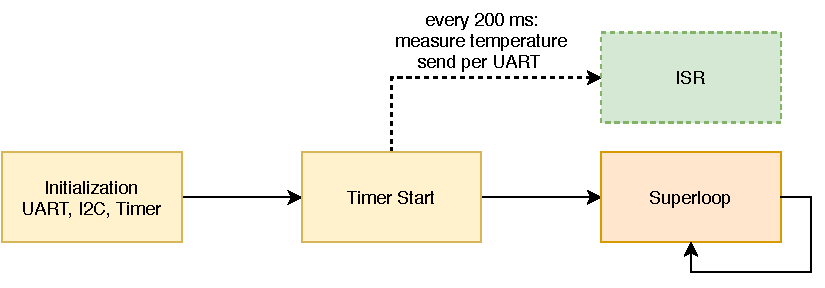
\includegraphics[width=0.75\textwidth]{img/swflow.pdf}
\end{figure}

A major chance is that instead of doing the expensive floating point calculations on the microcontroller, only the raw sensor data is sent to the PC. Here, the UI must do the necessary calculations to convert the raw sensor values to a human readable temperature. 

\subsection{Debugging the Microcontroller Code}

In order to be able to debug the microcontroller code, I added debugging functionality. There are two main parts to the debugging module. First, debugging is turned on an off in the file debug\_cfg.h. When debugging is on an LED connected to pin D6 of the microcontroller is initialized. This LED is off until the timer ISR starts, where it is toggled each time the ISR is executed. Further, error codes, if there are any errors, are transmitted through the UART. See the inline documentation for details. What I will mention here is that information about the initialization routines is sent when debugging is activated, as well as information about each step of the I2C process (if there are errors).

I use preprocessor flags to activate/deactivate the debugging. This makes the code a little hard to read, but is worth a lot when problems are encountered. One note here: The routine to interface with the MLX90614 always returns a status code. When debugging is off, this return value is simply ignored in the software in the current state.

\section{Hardware}

As a test platform I am using a cheap Arduino Nano clone, I have nothing else at my disposal. This has consequences for the project. First, I can't add the UART bluetooth module as I did in the proof of concept, the UART is already used on this board. I know that there is an Arduino software serial library to get around this, but I don't want to use a bit-banged UART (concerns about stability and speeds). Thus, the bluetooth module is gone, instead I am connecting per cable to the Nano to get the temperature values per serial interface.

As far as I2C is concerned, no external pullups are needed. The sensor features $10k\Omega$ pullups. The sensor is powered via the board's $3.3V$ output. The only other (not strictly necessary component) is the debug LED that does not need to be included and is deactivated once debugging mode is turned off. The complete setup is shown in fig. \ref{fig:hwsetup}. If a custom board would be made, the UART could be used for a bluetooth module as in the proof of concept. The only change in the software would be, if necessary, a different UART baudrate.

\begin{figure}[H]
  \caption{Hardware Setup.}
  \label{fig:hwsetup}
  \centering
    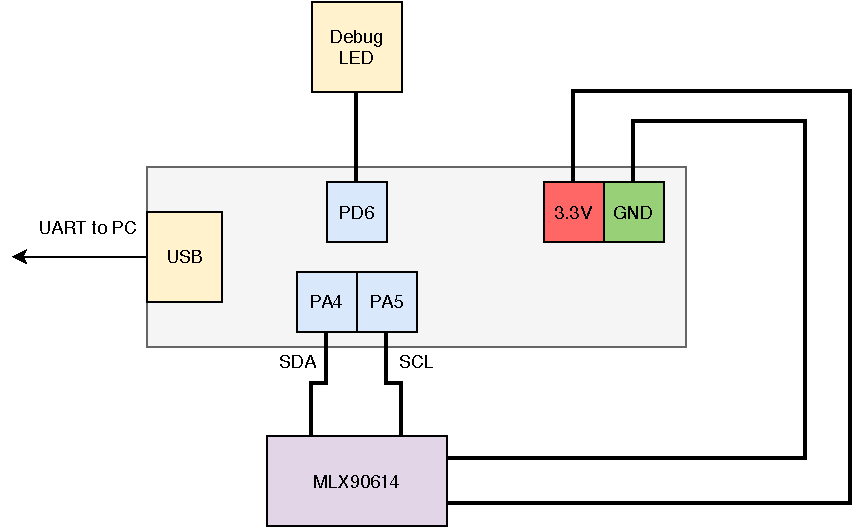
\includegraphics[width=0.75\textwidth]{img/hwsetup.pdf}
\end{figure}

\section{User Interface}

The user interface is still a hacked together mess and I am confident it could be done much better by someone with more experience in this area. However, it does it's job and that is to show the temperature currently being measured. In this new design iteration of the project, there are two interfacing scripts, both written in python. 

One script shows the sensor values as floating point numbers when started and has no graphical output. The graphical output script is pretty much the same as in the proof of concept, with two modifications: 

\begin{enumerate}
	\item The raw temperature value must be converted to a floating point value, as with the script showing the raw values.
	\item During the time temperature is measured, the mean value of all temperatures currently in the measurement window is calculated and displayed.
\end{enumerate}

The second point gets rid of any peaks and bumps and so on in a simple manner, providing the user of the project with a more stable temperature output. However, this only a quick, simple fix one can do. Maybe there is a better way to get a smooth output. 

An example of this is shown in fig. \ref{fig:ambienttemp} showing an ambient temperature measurement. The green dots are samples taken in $200ms$ intervals, the red line shows the average temperature over the measurement window. I can confirm the accuracy through an analog thermometer (more or less as it is analog).

\begin{figure}[H]
  \caption{Ambient Temperature Measurement.}
  \label{fig:ambienttemp}
  \centering
    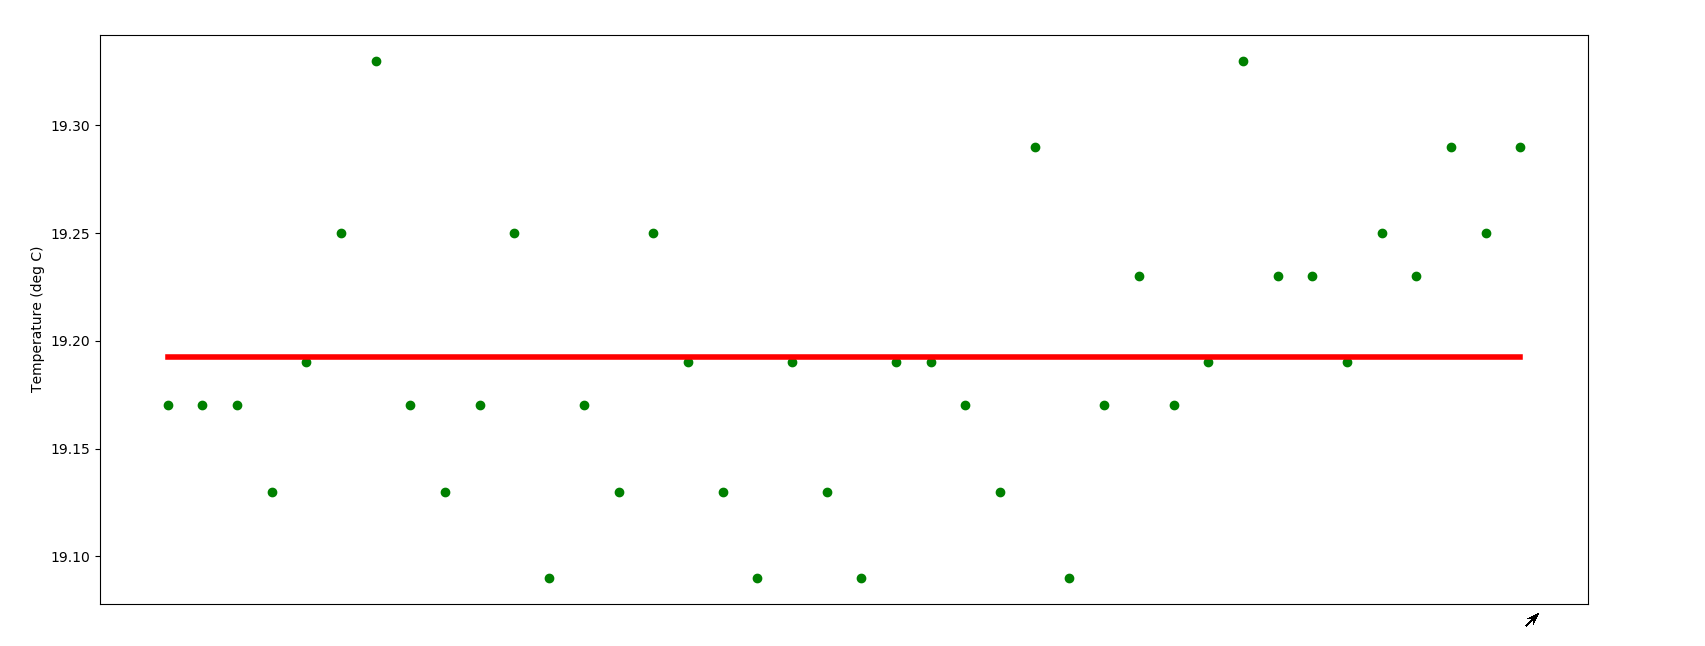
\includegraphics[width=0.75\textwidth]{img/ambienttemp.png}
\end{figure}

The next measurement is again a forehead measurement, depicted in fig. \ref{fig:foreheadtemp1}. Here, I measured for approximately $30$ seconds, with a distance of about 1-2 centimeters to the sensor.

\begin{figure}[H]
  \caption{Forehead Temperature Measurement 1.}
  \label{fig:foreheadtemp1}
  \centering
    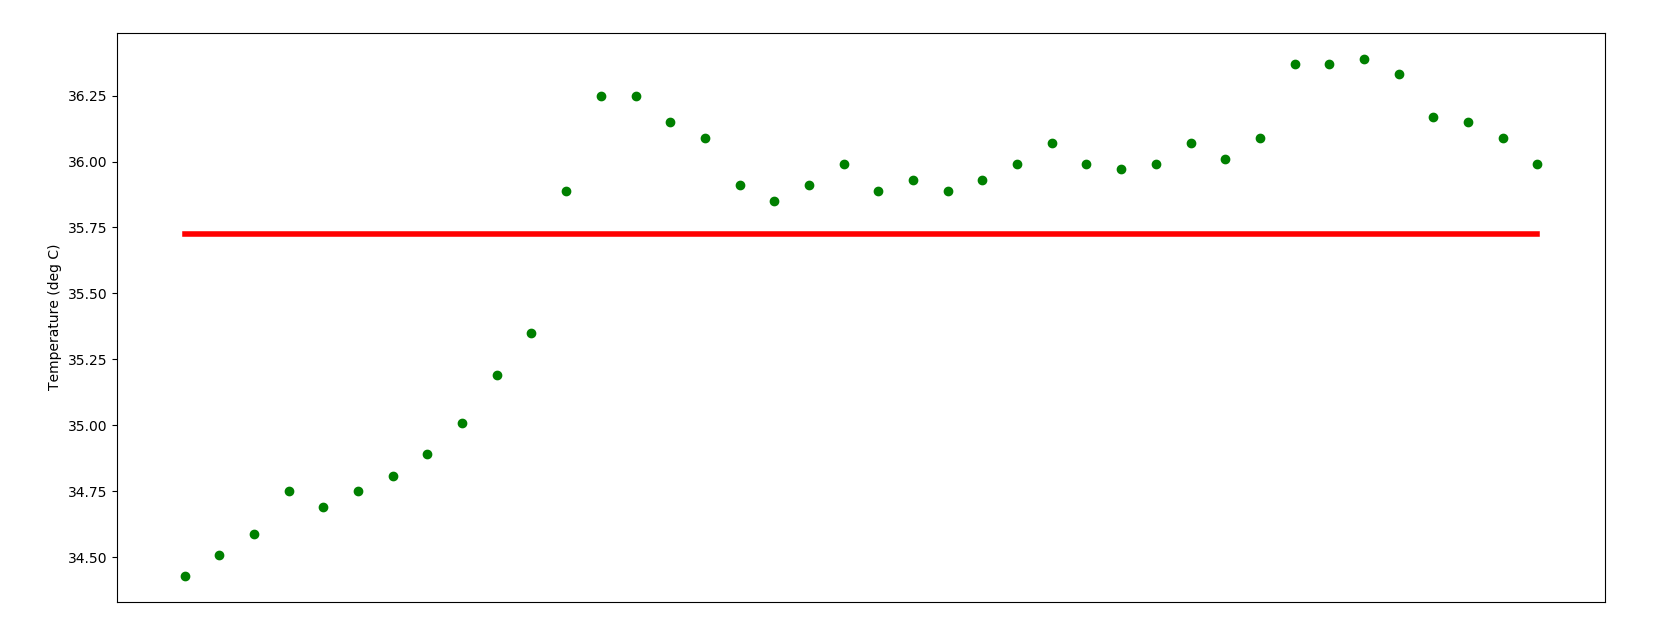
\includegraphics[width=0.75\textwidth]{img/foreheadtemp1.png}
\end{figure}

In fig. \ref{fig:foreheadtemp2} you can see that the measurement stabilizes after about $30-40$ seconds. 

\begin{figure}[H]
  \caption{Forehead Temperature Measurement 2.}
  \label{fig:foreheadtemp2}
  \centering
    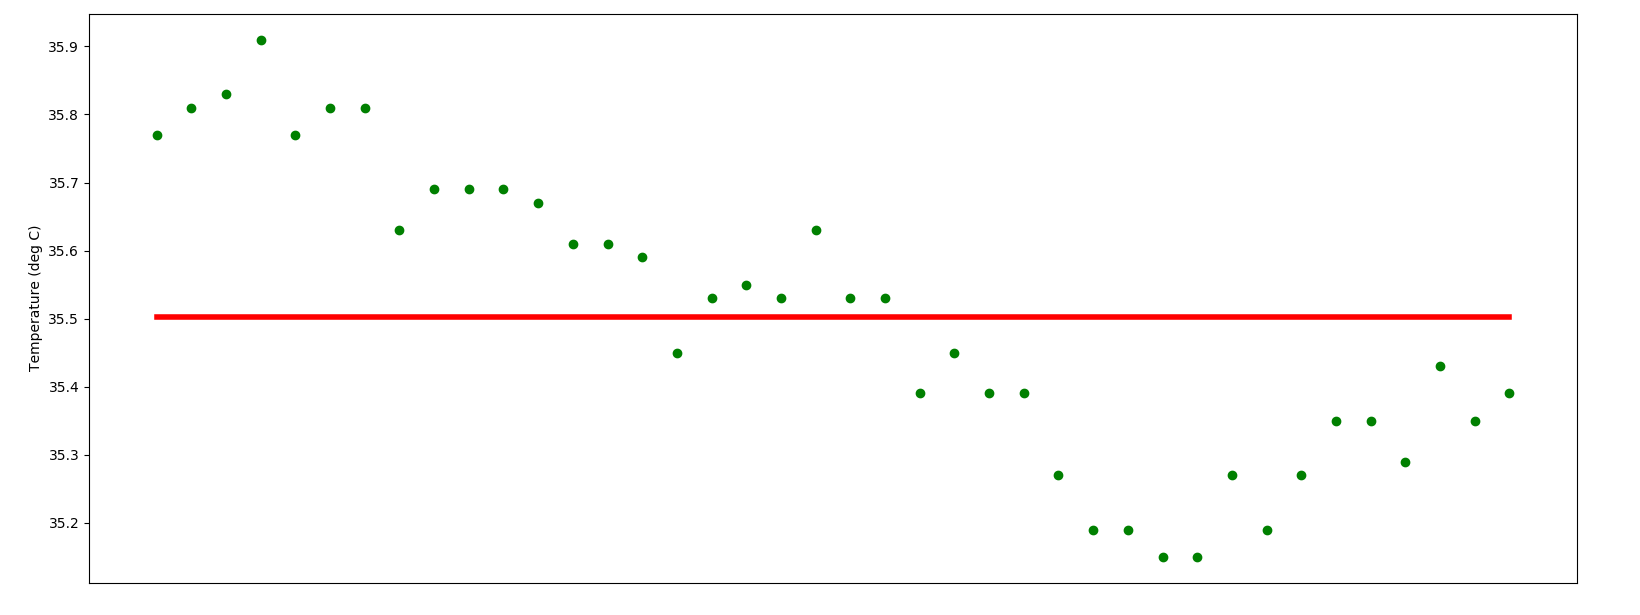
\includegraphics[width=0.75\textwidth]{img/foreheadtemp2.png}
\end{figure}

\section{Conclusion}

The software got simpler and smaller, the user interface is a little more readable. However, there is still more work to be done. I am confident the microcontroller application can function on a smaller microcontroller still. All in all, the current state of the project provides a stable base for future developments.

\section{Future Work}

First step is to get a nicer user interface, the second step is to further modify the microcontroller software for more efficiency. Another topic of interest is power consumption, especially for a battery powered version of the project in later design iterations. Further, a display connected directly to the microcontroller showing the measured temperatures may be an alternative to using a PC for showing the sensor data.



\end{document}